% !TEX root = paper.tex

\subsection{Simplifying Verification Conditions with Linear Types}\label{sec:encoding}

Potential aliasing of variable bindings in the presence of mutation
complicates verification~\cite{on-the-frame-problem}
because it requires explicitly reasoning about memory to determine the potential effects 
of each program statement. Given two bindings \verb`p` and \verb`q`, a predicate \verb`P(p)` about
the data reachable from \verb`p`,
and a statement \verb`S[q]` which mutates one of the memory locations reachable from \verb`q`,
if \verb`P(p)` is true before \verb`S[q]`, then \verb`P(p)` is guaranteed to remain true
after \verb`S[q]` if all the memory locations reachable from \verb`p` and \verb`q` are
disjoint.
Verus relies on the properties enforced by Rust's ``borrow checker'' to avoid explicit memory
reasoning: when encoding \verb`proof` and \verb`exec` function bodies
Verus treats the data associated with a uniquely-owned binding as an immutable value.
Mutable bindings are represented with single static assignment to immutable SMT constants,
one after each mutation.
We discuss Verus' encoding strategy with an example.

\begin{figure}
\makebox[0pt][l]{%
  \raisebox{-\totalheight}[0pt][0pt]{%
    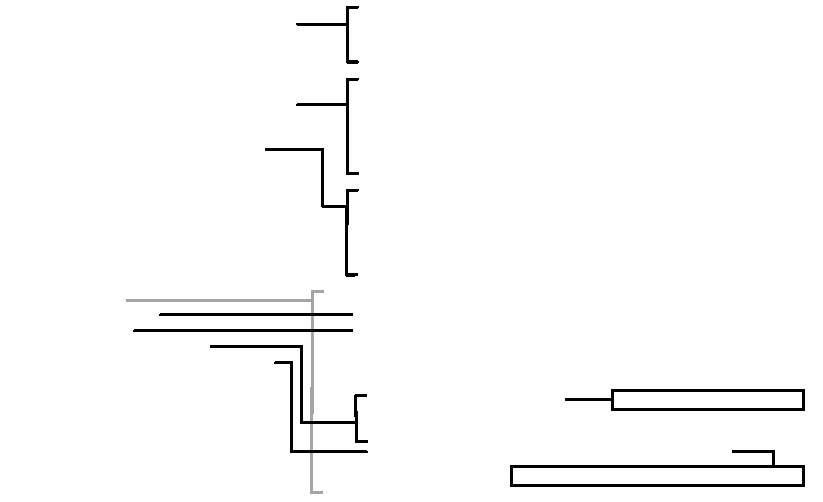
\includegraphics{encoding-example-overlay}}}%
\makebox[0pt][l]{%
  \raisebox{-\totalheight}[0pt][0pt]{%
  \begin{tikzpicture}[remember picture,overlay]
  \node[outer sep=0pt,inner sep=0pt] at (34em, -19.3em) {\lstinline[style=Verus]|VC: swap\_odd requires|};
          \node[outer sep=0pt,inner sep=0pt] at (31.7em, -22.9em) {\lstinline[style=Verus]|VC: assert(is\_odd(v) && is\_odd(w))|};
  \end{tikzpicture}%
    }}%
\begin{subfigure}[t]{.38\textwidth}
\vspace{.4em}
\begin{lstlisting}[language=Verus,style=VerusLineNos]
#[spec] fn is_odd(n: int) -> bool {
    n % 2 == 1
}

\end{lstlisting}
\vspace{.1em}
\begin{lstlisting}[language=Verus,style=VerusLineNos,firstnumber=5]
fn swap_odd(a: &mut u64, b: &u64) {
    requires((*old(a) as int + *b as %*\\*int) < u64::MAX &&
        is_odd(*b as int));
    ensures(is_odd(*a as int) ==
        !is_odd(*old(a) as int));
    *a = *a + *b;
}

\end{lstlisting}
\vspace{3.3em}
\begin{lstlisting}[language=Verus,style=VerusLineNos,firstnumber=13]
fn main() {
    let mut v = 0;
    let w = 3;
    swap_odd(&mut v, &w);
    assert(is_odd(v) && is_odd(w));
}
\end{lstlisting}
    \caption{Source of example}
    \end{subfigure}
    \hfill
    \begin{subfigure}[t]{.61\textwidth}
    \begin{lstlisting}[style=VerusLineNos]
(declare-fun is_odd.? (Poly) Bool) %*\lclnum\label{lclnum:smt:is-odd-decl}*
(assert (=> (forall ((n@ Poly)) %*\lclnum\label{lclnum:smt:is-odd-axiom}*
  (= (is_odd.? n@) (= (mod (%I n@) 2) 1)) %*\lclnum\label{lclnum:smt:is-odd-defn}*
...
(declare-fun req%swap_odd. (Int Int) Bool) %*\lclnum\label{lclnum:smt:swap_odd-req}*
(assert (forall ((pre%a@ Int) (b@ Int))
  (= (req%swap_odd. pre%a@ b@)
    (and
      (< (+ pre%a@ b@) 18446744073709551615)
      (is_odd.? (I b@))))))
...
(declare-fun ens%swap_odd. (Int Int Int) Bool) %*\lclnum\label{lclnum:smt:swap_odd-ens}*
(assert (forall ((pre%a@ Int) (a@ Int) (b@ Int))
  (= (ens%swap_odd. pre%a@ a@ %*\lclnum\label{lclnum:smt:swap_odd-req-pre}* b@) (and
    (uInv 64 a@) %*\lclnum\label{lclnum:smt:swap_odd-uInv}*
    (= (is_odd.? (I a@)) (not (is_odd.? (I pre%a@))))))))
...
(push)
(declare-const v@0 Int) (declare-const v@1 Int)
(declare-const w@ Int)
(assert (not %*\lclnum\label{lclnum:smt:falsifies}*
  (=> (= v@0 0) (=> (= w@ 3)
    (and
      (req%swap_odd. v@0 w@) %*\lclnum\label{lclnum:smt:main-req-vc}*
      (=> (uInv 64 v@1)
        (=> (ens%swap_odd. v@0 v@1 w@)
          (and (is_odd.? (I v@1)) (is_odd.? (I w@)))) %*\lclnum\label{lclnum:smt:main-assert-vc}*
    ))))))
(pop)
\end{lstlisting}
\caption{SMT-LIB encoding of the verification conditions for \texttt{main}.}
\end{subfigure}
    \caption{A simple example program and relevant parts of its encoding in Z3. The SMTLIB encoding
    has been slightly simplified to aid readability, but without compromising accuracy. In particular,
    we rename the constants, and we elide the patterns chosen for quantifier instantiation in Z3~\cite{e-matching},
    some temporary variables used to optimize the SMT encoding, and some facilities for error reporting.} \label{fig:encoding-example}
\end{figure}

\autoref{fig:encoding-example} shows a simple program, and how Verus encodes it into SMT-LIB~\cite{smtlib}, the input to Z3.
First let us dispatch some boilerplate that clutters the figure.
The functions \verb`%I`, \verb`I` and the sort \verb`Poly` appear often. They are part of the polymorphism encoding machinery of Verus,
which is inspired by Boogie\cite{poly-boogie}. Function \verb`I` is a cast from \verb`Int` to \verb`Poly`, a Z3 sort
representing a polymorphic type, and \verb`%I` is a cast from \verb`Poly` to \verb`Int`. \verb`spec` function arguments
are always \verb`Poly` due to interactions with the Z3's quantifier instantiation.
\verb`uInv 64` \clref{lclnum:smt:swap_odd-uInv} is a typing invariant that restrict the SMT \verb`Int`
type to the range of Rust's \verb`u64` machine type.

In SMT-LIB, functions are defined by constructing axioms (e.g. \clref{lclnum:smt:is-odd-axiom})
that relate their declaration (e.g. \clref{lclnum:smt:is-odd-decl}) to their definition (e.g. \clref{lclnum:smt:is-odd-defn}).
Verus' \verb`spec` is designed to closely match SMT logic, enabling the straightforward encoding of \verb`is_odd`~\clref{lclnum:smt:is-odd-defn}.
Similarly, the SMT functions representing the precondition and postcondition for \verb`swap_odd` (
\verb`req%swap_odd.` \clref{lclnum:smt:swap_odd-req} and \verb`ens%swap_odd.` \clref{lclnum:smt:swap_odd-ens} respectively)
closely match their corresponding \verb`spec`-mode Verus code.
The mutable reference \verb`a: &mut u64` is represented as a pair of constants, \verb`pre%a@` and \verb`a@` \clref{lclnum:smt:swap_odd-req-pre},
respectively the initial and final value. The immutable reference (\verb`b: &u64`) is represented as a single constant \verb`b@`.
Reference types (\verb`&mut` and \verb`&`) do not need special treatment
thanks to the borrow checker's guarantees:
for example the arguments \verb`a` and \verb`b` cannot be aliased because mutable and immutable
references to the same data cannot exist at the same time.

The last SMT-LIB fragment is the encoding of the \verb`main` function and its associated verification conditions.
Like other tools, Verus encodes its proof search as a query to Z3 to find an assignment to constants that
falsifies \clref{lclnum:smt:falsifies} verification conditions: an \verb`unsat` result is a proof that such assignment does not
exist, i.e. verification succeeded.
The constants \verb`v@0` and \verb`v@1` represent the value of binding \verb`v` before and after the call to
\verb`swap_odd`, and \verb`w` represents the immutable binding \verb`w`.
The call to \verb`swap_odd` is encoded modularly with a verification condition to check its precondition \clref{lclnum:smt:main-req-vc}.

Another call to \verb`ens%swap_odd.` introduces its postcondition as an antecedent for all future verification
conditions in the function.
Thanks to Rust's linear type system, there is no need to explicitly model the heap here: the two arguments to \verb`swap_odd`
are guaranteed to point to distinct regions of memory.
Finally, the \verb`assert` is encoded as part of the verification condition \clref{lclnum:smt:main-assert-vc}.


